%
% main.tex
%
% Copyright (C) 2022 by SpaceLab.
%
% Camera Payload Preliminary Design Review
%
% This work is licensed under the Creative Commons Attribution-ShareAlike 4.0
% International License. To view a copy of this license,
% visit http://creativecommons.org/licenses/by-sa/4.0/.
%

%
% \brief Main file.
%
% \author Gabriel Mariano Marcelino <gabriel.mm8@gmail.com>
% \author Bruno Benedetti <brunobenedetti45@gmail.com>
%
% \version 0.1.0
%
% \date 2022/06/24
%

\documentclass{beamer}

\usepackage{presentation}

\title[Presentation]{SpaceLab ADCS Module - PDR}
\author[SpaceLab]{Rebecca Q. Do Ó, Bruno Benedetti, Caique S. de M. Gomes, Gabriel M. Marcelino, André M. P. de Mattos, Matheus Wagner}
\institute[]{SpaceLab - UFSC}
\date{2022 August 2}

\hypersetup
{
    pdfauthor	= {SpaceLab},
    pdfsubject	= {PDR of a ADCS controller module},
    pdftitle	= {\title},
    pdfkeywords	= {Nanosatellites, CubeSats, ADCS}
}

\begin{document}

    %
% titlepage.tex
%
% Copyright (C) 2022 by SpaceLab.
%
% Camera Payload Preliminary Design Review
%
% This work is licensed under the Creative Commons Attribution-ShareAlike 4.0
% International License. To view a copy of this license,
% visit http://creativecommons.org/licenses/by-sa/4.0/.
%

%
% \brief Title page.
%
% \author Gabriel Mariano Marcelino <gabriel.mm8@gmail.com>
% \author Vitória Beatriz Bianchin <vitoriabbianchin@gmail.com>
% \author Caique Sales de Miranda Gomes <kiqsmg@gmail.com>
%
% \version 0.1.0
%
% \date 2022/06/24
%

\begin{frame}
    \titlepage
\end{frame}
    %
% contents.tex
%
% Copyright (C) 2022 by SpaceLab.
%
% Camera Payload Preliminary Design Review
%
% This work is licensed under the Creative Commons Attribution-ShareAlike 4.0
% International License. To view a copy of this license,
% visit http://creativecommons.org/licenses/by-sa/4.0/.
%

%
% \brief Table of contents.
%
% \author Gabriel Mariano Marcelino <gabriel.mm8@gmail.com>
% \author Vitória Beatriz Bianchin <vitoriabbianchin@gmail.com>
% \author Caique Sales de Miranda Gomes <kiqsmg@gmail.com>
%
% \version 0.1.0
%
% \date 2022/06/24
%

\begin{frame}
    \frametitle{Summary}
    \tableofcontents
\end{frame}

    
    \begin{frame}
        \titlepage
    \end{frame}

    \begin{frame}
        \frametitle{Summary}
        \tableofcontents
    \end{frame}
    
    \section{Project Overview}

        %
% introduction.tex
%
% Copyright (C) 2022 by SpaceLab.
%
% Camera Payload Preliminary Design Review
%
% This work is licensed under the Creative Commons Attribution-ShareAlike 4.0
% International License. To view a copy of this license,
% visit http://creativecommons.org/licenses/by-sa/4.0/.
%

%
% \brief Introduction slides.
%
% \author Gabriel Mariano Marcelino <gabriel.mm8@gmail.com>
% \author Vitória Beatriz Bianchin <vitoriabbianchin@gmail.com>
% \author Caique Sales de Miranda Gomes <kiqsmg@gmail.com>
%
% \version 0.1.0
%
% \date 2022/06/24
%

\begin{frame}{Proposal and Objectives}
    
    \begin{columns}[t]
        \begin{column}[t]{0.65\textwidth}
            \begin{itemize}
                \item ADCS (Attitude Determination and Control System) Module
                \vspace{0.5cm}
                \item Project name: ``\textit{ADCS Module}''
                \vspace{0.5cm}
                \item Main objective: Create a module with basic instrumentation for an active magnetic ADCS system 
            \end{itemize}
        \end{column}
        \begin{column}[t]{0.4\textwidth}
            \begin{figure}[!ht]
                \begin{center}
                    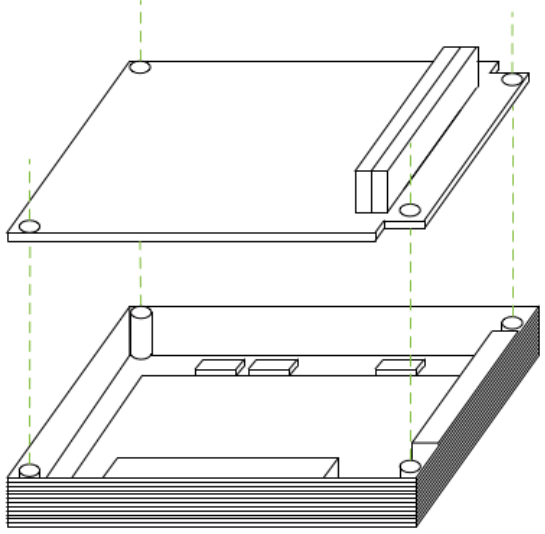
\includegraphics[width=4cm]{figures/adcs-module-idea.png}
                \end{center}
            \end{figure}
        \end{column}
    \end{columns}
    
\end{frame}

\begin{frame}{Requirements}

    \begin{itemize}
        \item \textbf{SLB-ADCS-REQ-001:} The module must be compliant with CubeSat and PC-104 standards; 
        \item \textbf{SLB-ADCS-REQ-002:} The module should be designed for 3U CubeSats (considering soft requirements for stabilization);
        \item \textbf{SLB-ADCS-REQ-003:} The module must include compact magnetic coils on 3-axis;
        \item \textbf{SLB-ADCS-REQ-004:} The module must have a microcontroller with sufficient performance for basic ADCS algorithms;  
        \item \textbf{SLB-ADCS-REQ-005:} The module must include built-in sensors: magnetometer (3-axis), gyroscope (3-axis), voltage/current (each coil), temperature (each coil), and sun sensor (photodiode interfaces for 3-axis); 
    \end{itemize}

\end{frame}

\begin{frame}{Requirements}

    \begin{itemize}
        \item \textbf{SLB-ADCS-REQ-006:} The module must have current (H-bridge) drivers with a safe operation for the magnetic coils;  
        \item \textbf{SLB-ADCS-REQ-007:} The module should assume moderate power consumption during stabilization;
        \item \textbf{SLB-ADCS-REQ-008:} The power circuits must have overcurrent/overvoltage/overtemperature protection (fuses, load switches, overtemperature shutdown, ...); 
        \item \textbf{SLB-ADCS-REQ-009:} The board should be designed to minimize overheating elements and mixing digital/analog/power circuits;    
        \item \textbf{SLB-ADCS-REQ-010:} The board should have 4 layers, including continuous power planes for better electrical/heat/noise performance.
    \end{itemize}

\end{frame}
        
    \begin{frame}{Overview}

    \begin{columns}[t]
        \begin{column}[t]{0.5\textwidth}
            \begin{itemize}
                \item Attitude Determination and Control System (ADCS) module for small satellites (Cubesat)
                \vspace{0.3cm}
                \item Custom made project
                \vspace{0.3cm}
                \item Fully open source

            \end{itemize}
        \end{column}
        \begin{column}[t]{0.5\textwidth}
            \begin{figure}[!ht]
                \begin{center}
                    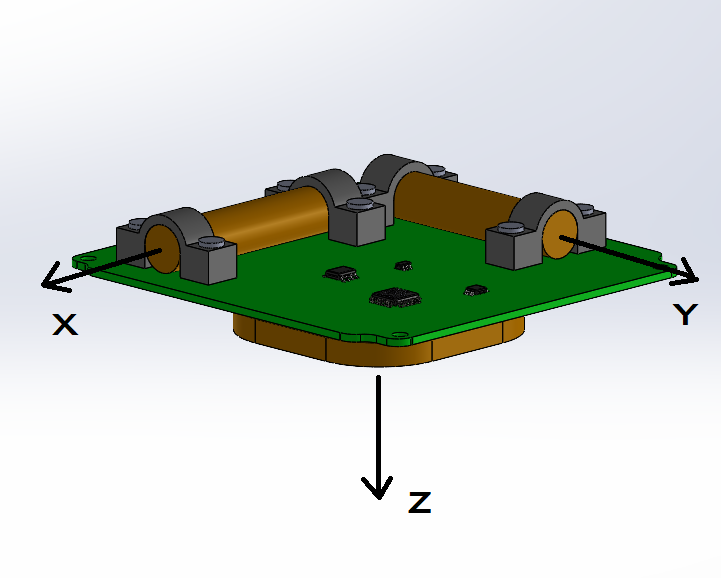
\includegraphics[width=5.5cm]{figures/Image axles.png}
                \end{center}
            \end{figure}
        \end{column}
    \end{columns}

\end{frame}

    \begin{frame}{Overview}

    \begin{columns}[t]
        \begin{column}[t]{0.9\textwidth}
            \begin{itemize}
                \item Main objective: Create a module with
basic instrumentation for an active
magnetic ADCS
                \vspace{0.3cm}
                \item Three-axis actuators: two
magnetorquers with
magnetic core and one with
air core; Nominal dipole
strength: $0.2 Am^2$ \textcolor{red}{TBC}.
                \vspace{0.3cm}
                \item Current, Voltage and Temperature sensors for each magnetorquer;

            \end{itemize}
        \end{column}
    \end{columns}

\end{frame}

    \section{Related Projects and References}

        %
% related-work.tex
%
% Copyright (C) 2022 by SpaceLab.
%
% Camera Payload Preliminary Design Review
%
% This work is licensed under the Creative Commons Attribution-ShareAlike 4.0
% International License. To view a copy of this license,
% visit http://creativecommons.org/licenses/by-sa/4.0/.
%

%
% \brief Introduction slides.
%
% \author Gabriel Mariano Marcelino <gabriel.mm8@gmail.com>
% \author Vitória Beatriz Bianchin <vitoriabbianchin@gmail.com>
% \author Caique Sales de Miranda Gomes <kiqsmg@gmail.com>
%
% \version 0.1.0
%
% \date 2022/06/24
%


\begin{frame}{Comercial ADCS modules for CubeSats}

    A few commercial ADCS modules for CubeSats are available in the market:

    \begin{itemize}
        \item \href{https://www.isispace.nl/product/isis-magnetorquer-board/}{\textcolor{blue}{\underline{ISIS - iMTQ Magnetorquer Board}}}
        \vspace{0.4cm}
        \item \href{https://gomspace.com/shop/subsystems/attitude-orbit-control-systems/nanotorque-gst-600.aspx}{\textcolor{blue}{\underline{GomSpace - NanoTorque GST-600}}}
        \vspace{0.4cm}
        \item \href{https://nanoavionics.com/cubesat-components/cubesat-magnetorquer-satbus-mtq/}{\textcolor{blue}{\underline{NanoAvionics - CubeSat Magnetorquer SatBus MTQ}}}
        \vspace{0.4cm}
        \item \href{}{\textcolor{blue}{\underline{...}}}
    \end{itemize}

\end{frame}

% #########################################################################
% #########################################################################

\begin{frame}{Comercial ADCS: \href{https://www.isispace.nl/product/isis-magnetorquer-board/}{\textcolor{cyan}{\underline{ISIS - iMTQ Magnetorquer Board}}}}

    \begin{columns}[t]
        \begin{column}[t]{0.5\textwidth}
            \begin{itemize}
                \item Three-axis actuators: two magnetorquers with magnetic core and one with air core; Nominal dipole strength: $0.2 Am^2$;
                \item Current and temperature sensors for each magnetorquer;
                \item Suitable to detumble up to 12U (~24kg) CubeSats.
            \end{itemize}
        \end{column}
        \begin{column}[t]{0.5\textwidth}
            \begin{figure}[!ht]
                \begin{center}
                    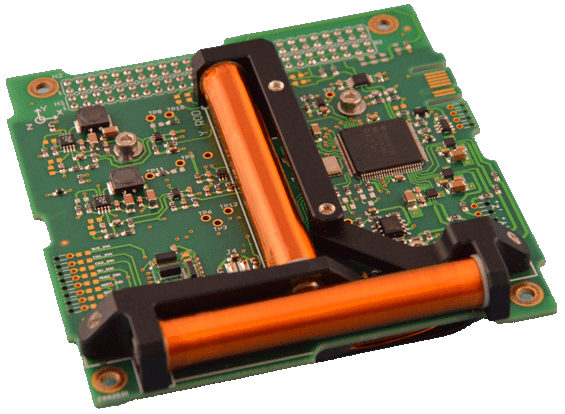
\includegraphics[width=4.5cm]{figures/magnetorquers-isis.png}
                \end{center}
            \end{figure}
        \end{column}
    \end{columns}

    

    
\end{frame}

\begin{frame}{Comercial Coils: \href{https://gomspace.com/shop/subsystems/attitude-orbit-control-systems/nanotorque-gst-600.aspx}{\textcolor{cyan}{\underline{GomSpace - NanoTorque GST-600}}}}

    \begin{columns}[t]
        \begin{column}[t]{0.5\textwidth}
            \begin{itemize}
                \item 3-axis magnetorquer;
                \item Torque $>0.3 Am^2$ per axis;
                \item Build-in temperature sensor;
                \item High torque and low residual dipole.
            \end{itemize}
        \end{column}
        \begin{column}[t]{0.5\textwidth}
            \begin{figure}[!ht]
                \begin{center}
                    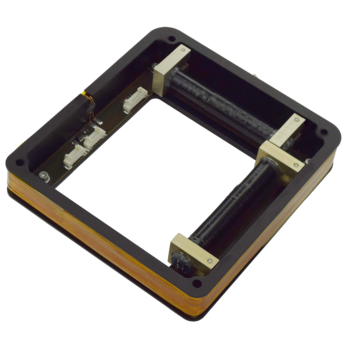
\includegraphics[width=4.5cm]{figures/magnetorquers-gomspace.png}
                \end{center}
            \end{figure}
        \end{column}
    \end{columns}
    
\end{frame}

% #########################################################################
% #########################################################################

\begin{frame}{Comercial Coils: \href{https://nanoavionics.com/cubesat-components/cubesat-magnetorquer-satbus-mtq/}{\textcolor{cyan}{\underline{NanoAvionics - CubeSat Magnetorquer MTQ}}}}

    \begin{columns}[t]
        \begin{column}[t]{0.5\textwidth}
            \begin{itemize}
                \item 2 magnetorquer rods with soft magnetic cores and 1 coil with air core;
                \item Dipole magnetic moment strength: $0.3 Am^2$ (X/Y axis), $0.34 Am^2$ (Z axis);
                \item Supply voltage: up to 5 V;
                \item Power consumption: 0.4 W.
            \end{itemize}
        \end{column}
        \begin{column}[t]{0.5\textwidth}
            \begin{figure}[!ht]
                \begin{center}
                    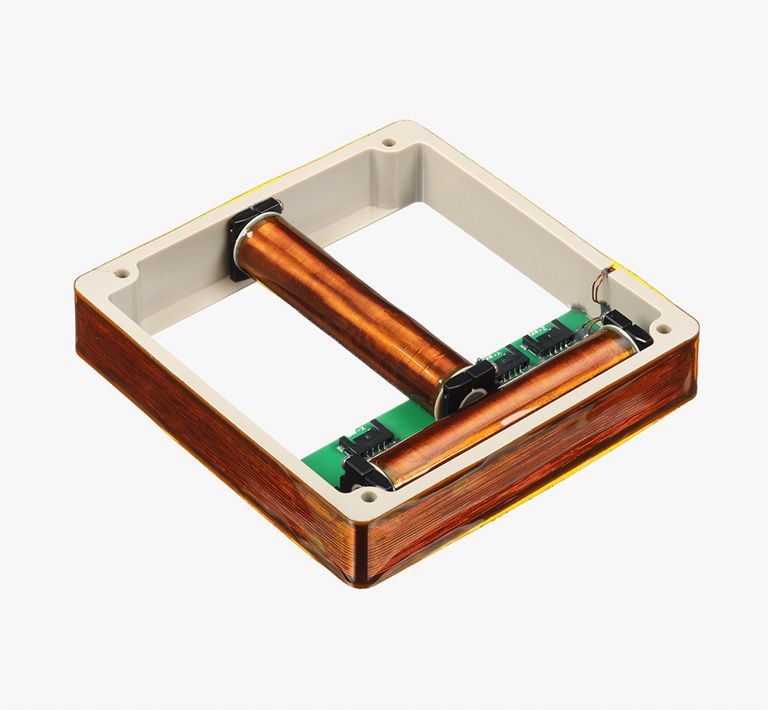
\includegraphics[width=4.5cm]{figures/magnetorquers-nanoavionics.png}
                \end{center}
            \end{figure}
        \end{column}
    \end{columns}
    
\end{frame}
        
\begin{frame}{Comercial ADCS modules for CubeSats}

    A few commercial ADCS modules for CubeSats are available in the market:

    \begin{itemize}
        \item \href{https://www.isispace.nl/product/isis-magnetorquer-board/}{\textcolor{blue}{\underline{ISIS - iMTQ Magnetorquer Board}}}
        \vspace{0.4cm}
        \item \href{https://gomspace.com/shop/subsystems/attitude-orbit-control-systems/nanotorque-gst-600.aspx}{\textcolor{blue}{\underline{GomSpace - NanoTorque GST-600}}}
        \vspace{0.4cm}
        \item \href{https://nanoavionics.com/cubesat-components/cubesat-magnetorquer-satbus-mtq/}{\textcolor{blue}{\underline{NanoAvionics - CubeSat Magnetorquer SatBus MTQ}}}
        \vspace{0.4cm}
        \item \href{}{\textcolor{blue}{\underline{...}}}
    \end{itemize}

\end{frame}

% #########################################################################
% #########################################################################

\begin{frame}{Comercial ADCS: \href{https://www.isispace.nl/product/isis-magnetorquer-board/}{\textcolor{cyan}{\underline{ISIS - iMTQ Magnetorquer Board}}}}

    \begin{columns}[t]
        \begin{column}[t]{0.5\textwidth}
            \begin{itemize}
                \item Three-axis actuators: two magnetorquers with magnetic core and one with air core; Nominal dipole strength: $0.2 Am^2$;
                \item Current and temperature sensors for each magnetorquer;
                \item Suitable to detumble up to 12U (~24kg) CubeSats.
            \end{itemize}
        \end{column}
        \begin{column}[t]{0.5\textwidth}
            \begin{figure}[!ht]
                \begin{center}
                    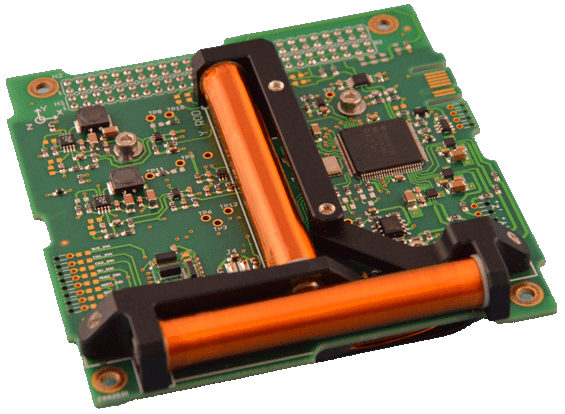
\includegraphics[width=4.5cm]{figures/magnetorquers-isis.png}
                \end{center}
            \end{figure}
        \end{column}
    \end{columns}

    

    
\end{frame}

\begin{frame}{Comercial Coils: \href{https://gomspace.com/shop/subsystems/attitude-orbit-control-systems/nanotorque-gst-600.aspx}{\textcolor{cyan}{\underline{GomSpace - NanoTorque GST-600}}}}

    \begin{columns}[t]
        \begin{column}[t]{0.5\textwidth}
            \begin{itemize}
                \item 3-axis magnetorquer;
                \item Torque $>0.3 Am^2$ per axis;
                \item Build-in temperature sensor;
                \item High torque and low residual dipole.
            \end{itemize}
        \end{column}
        \begin{column}[t]{0.5\textwidth}
            \begin{figure}[!ht]
                \begin{center}
                    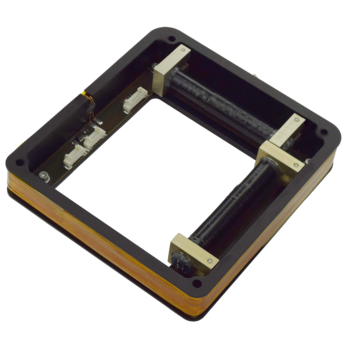
\includegraphics[width=4.5cm]{figures/magnetorquers-gomspace.png}
                \end{center}
            \end{figure}
        \end{column}
    \end{columns}
    
\end{frame}

% #########################################################################
% #########################################################################

\begin{frame}{Comercial Coils: \href{https://nanoavionics.com/cubesat-components/cubesat-magnetorquer-satbus-mtq/}{\textcolor{cyan}{\underline{NanoAvionics - CubeSat Magnetorquer MTQ}}}}

    \begin{columns}[t]
        \begin{column}[t]{0.5\textwidth}
            \begin{itemize}
                \item 2 magnetorquer rods with soft magnetic cores and 1 coil with air core;
                \item Dipole magnetic moment strength: $0.3 Am^2$ (X/Y axis), $0.34 Am^2$ (Z axis);
                \item Supply voltage: up to 5 V;
                \item Power consumption: 0.4 W.
            \end{itemize}
        \end{column}
        \begin{column}[t]{0.5\textwidth}
            \begin{figure}[!ht]
                \begin{center}
                    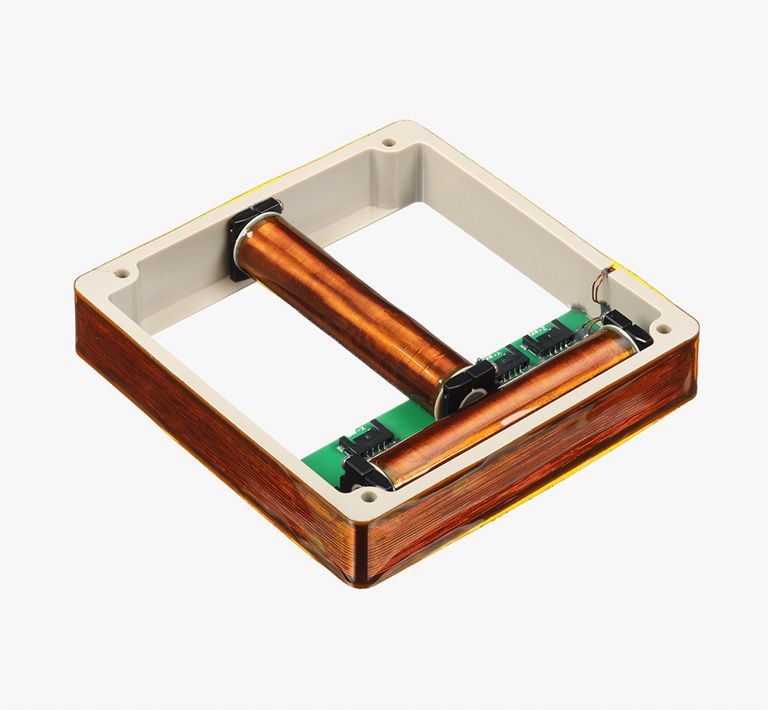
\includegraphics[width=4.5cm]{figures/magnetorquers-nanoavionics.png}
                \end{center}
            \end{figure}
        \end{column}
    \end{columns}
    
\end{frame}
        
\section{Preliminary Design}

\begin{frame}{Specifications}

    \begin{itemize}
        \item Microcontroller: STM32F303RCT6 
        \item Sensors:
        \begin{itemize}
            \item Voltage sensor (4x)
            \item Current sensor (4x)
            \item Temperature sensor (4x)
            \item Gyroscope (3-axis)
            \item Magnetometer (3-axis)
            \item Sun sensors (?x)
        \end{itemize}
        \item H-bridge (3x)
        \item Interfaces: CAN and SPI \textcolor{red}{TBC}
        \item Mass: \textcolor{red}{TBD}
        \item PC-104 compatible
    \end{itemize}

\end{frame}

\begin{frame}{Features}
    \begin{columns}[t]
        \begin{column}[t]{0.5\textwidth}
        \item Module Capabilities
        \vspace{0.3cm}
            \begin{itemize}
                \item Detumbling
                \vspace{0.3cm}
                \item Pointing
                \vspace{0.3cm}
                \item Idle
                \vspace{0.3cm}
            \end{itemize}
        \end{column}
        \begin{column}[t]{0.5\textwidth}
            \begin{figure}[!ht]
                \begin{center}
                    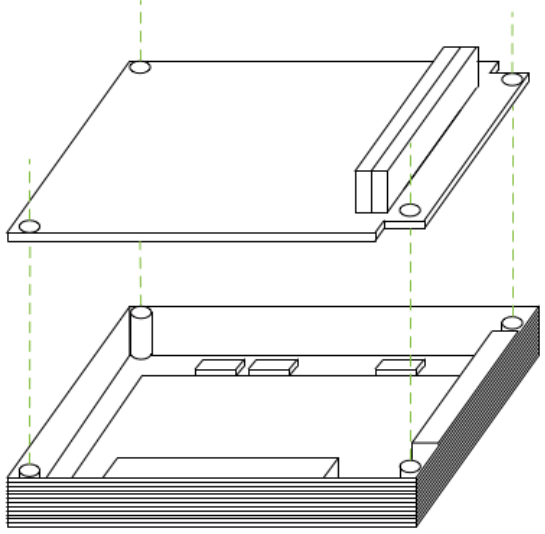
\includegraphics[width=5.5cm]{figures/adcs-module-idea.png}
                \end{center}
            \end{figure}
        \end{column}
    \end{columns}
\end{frame}

\begin{frame}{Electrical Block Diagram}

    \begin{figure}[!ht]
        \begin{center}
            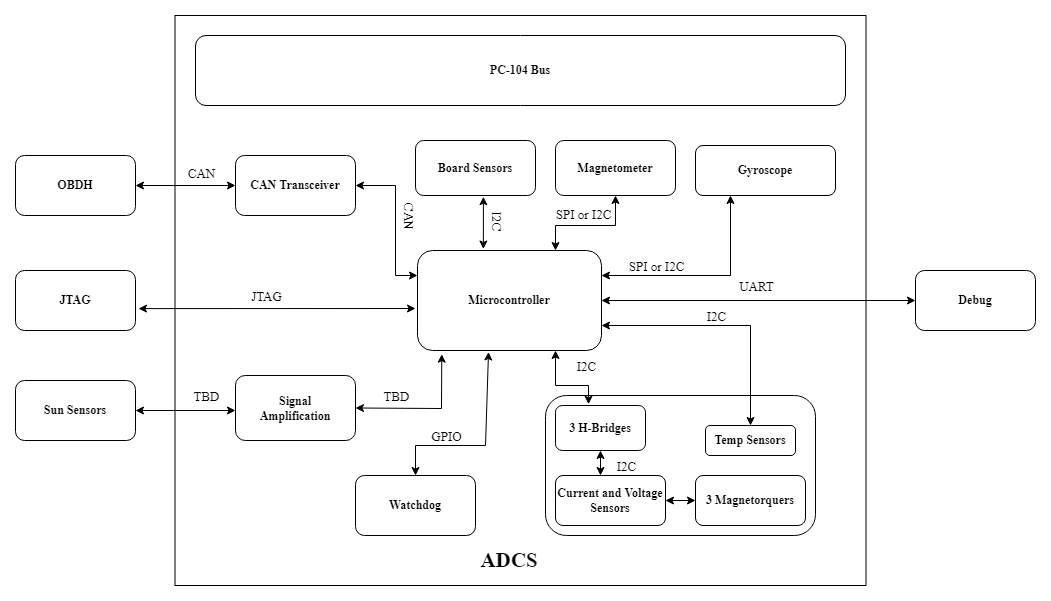
\includegraphics[width=11cm]{figures/ADCS.drawio (2).png}
        \end{center}
    \end{figure}

\end{frame}

\begin{frame}{Magnetorquer Loop Control Diagram}

    \begin{figure}[!ht]
        \begin{center}
            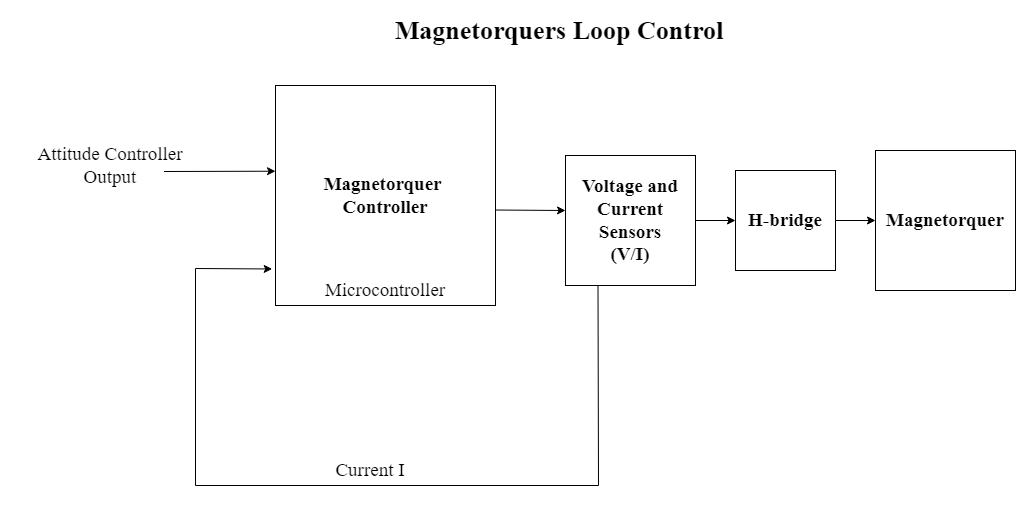
\includegraphics[width=11cm]{figures/Malha_Magnetorquers.drawio (2).png}
        \end{center}
    \end{figure}

\end{frame}

\begin{frame}{Detumbling Loop Control Diagram}

    \begin{figure}[!ht]
        \begin{center}
            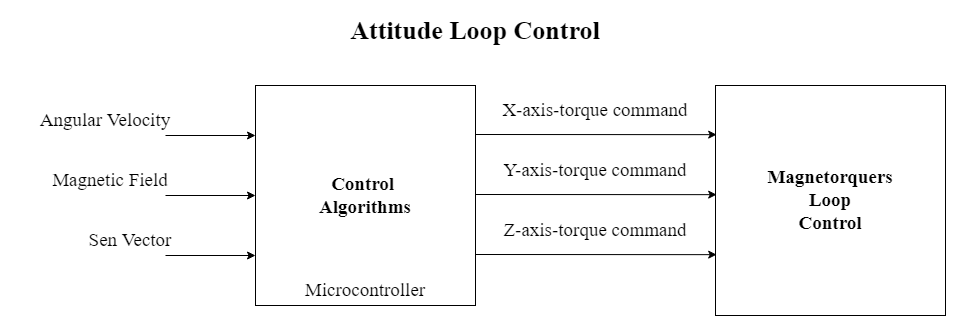
\includegraphics[width=11cm]{figures/Malha_Attitude_controller.drawio.png}
        \end{center}
    \end{figure}

\end{frame}

\begin{frame}{Possible Hardware for the mission}

    \begin{itemize}
        \item Voltage and current sensor - ina226 (4x) 
        \item Temperature sensor - TMP100 (4x)
        \item Gyroscope (3-axis) -  I3G4250DTR (1x)
        \item Magnetometer (3-axis) - MMC5983MA (1x)
        \item H-bridge - DRV8834PWP (3x) \textcolor{red}{TBC}
        \item Sun sensors - (?x) \textcolor{red}{TBC}
    \end{itemize}

\end{frame}

\begin{frame}{Sensors}

    \begin{table}[!htb]\scriptsize
    \centering
    \label{tab:cost-estimation}
    \begin{tabular}{lccc}
        \toprule[1.5pt]
        \textbf{Characteristic} & \textbf{ina226} & \textbf{TPM100} & \textbf{MMC5983MA} \\
        \midrule
        Manufacturer        &  Texas Instruments & Texas Instruments  & MEMSIC  \\
        Partnumber          & INA226AIDGSR & TMP100MDBVREP & MMC5983MA \\
        Interface           & I2C    & I2C & SPI or I2C\\
        Temperature range   & –40°C a 125°C & –55°C to 125°C & -40°C to +105°C \\        
        \bottomrule[1.5pt]
    \end{tabular}
\end{table}

\end{frame}

\begin{frame}{Sensors}

    \begin{table}[!htb]\scriptsize
    \centering
    \label{tab:cost-estimation}
    \begin{tabular}{lccc}
        \toprule[1.5pt]
        \textbf{Characteristic} & \textbf{I3G4250D} & \textbf{Sun sensor} \\
        \midrule
        Manufacturer     &  MEMSIC & -  \\
        Partnumber       & I3G4250DTR & - \\
        Interface        & SPI or I2C    & - \\
        Temperature range   & -40 °C to +85 °C & - \\
        
        \bottomrule[1.5pt]
    \end{tabular}
\end{table}

\end{frame}

\begin{frame}{External Watchdog}

    \begin{itemize}
        \item IC: Texas Instruments TPS3823
        \vspace{0.5cm}
        \item Voltage monitor with a watchdog timer feature
        \vspace{0.5cm}
        \item Timeout period: $1600\ ms$
        \vspace{0.5cm}
    \end{itemize}

\end{frame}

% #########################################################################
% #########################################################################

\begin{frame}{Bill of Materials\footnote{2 units.}}

\begin{table}[!htb]\scriptsize
    \centering
    \label{tab:cost-estimation}
    \begin{tabular}{lccc}
        \toprule[1.5pt]
        \textbf{Component} & \textbf{Description} & \textbf{Partnumber} & \textbf{Quantity} \\
        \midrule
        Microcontroller       &  - & STM32F303RCT6  & 2 \\
        CAN Transceiver       & - & TCAN330GD  & 2 \\
        Voltage and Current Sensors   & - & ina226 & 8\\
        Temperature Sensors   & - & TMP100 & 8\\
        Gyroscope             & - & I3G4250DTR & 2\\
        Magnetometer          & - & MMC5983MA & 2\\
        Sun sensors           & - & \textcolor{red}{TBD} & \textcolor{red}{TBD}\\
        H-Bridge              & - & \textcolor{red}{TBD} & 6 \\
        Copper wire           & \textcolor{red}{TBD} & - & 1 \\
        Magnetic core         & \textcolor{red}{TBD} & - & 4 \\
        Watchdog              & - & TPS3823 & 2 \\
        
        \bottomrule[1.5pt]
    \end{tabular}
\end{table}

\end{frame}

\begin{frame}{Dimensions}
    
    \begin{figure}[!ht]
        \begin{center}
            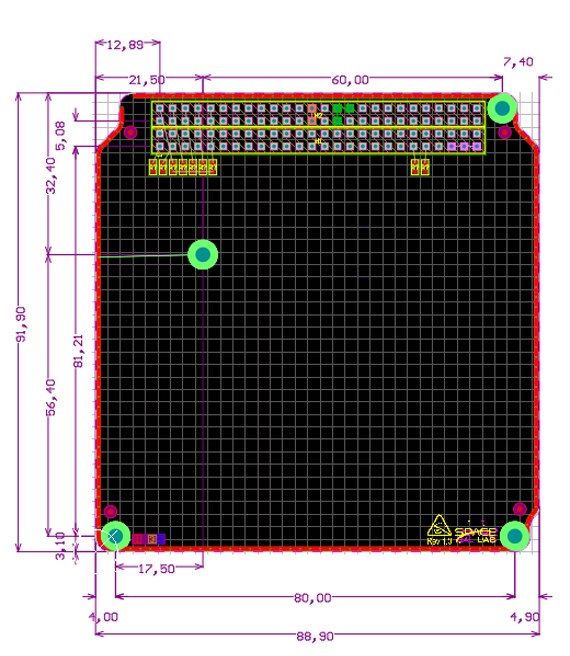
\includegraphics[width=6cm]{figures/board-dimensions-adcs.png}
        \end{center}
    \end{figure}

\end{frame}

\begin{frame}{Dimensioning: ADCS structure}
    
     \begin{columns}[t]
        \begin{column}[t]{0.5\textwidth}
            \begin{itemize}
                \item Limiting factors:
                     \item 3U cubesat
                \item The sizing must take in account the Z axle for the dimensioning limits
                     \item Estimated space available: (90x90x40mm)

            \end{itemize}
        \end{column}
        \begin{column}[t]{0.5\textwidth}
            \begin{figure}[!ht]
                \begin{center}
                    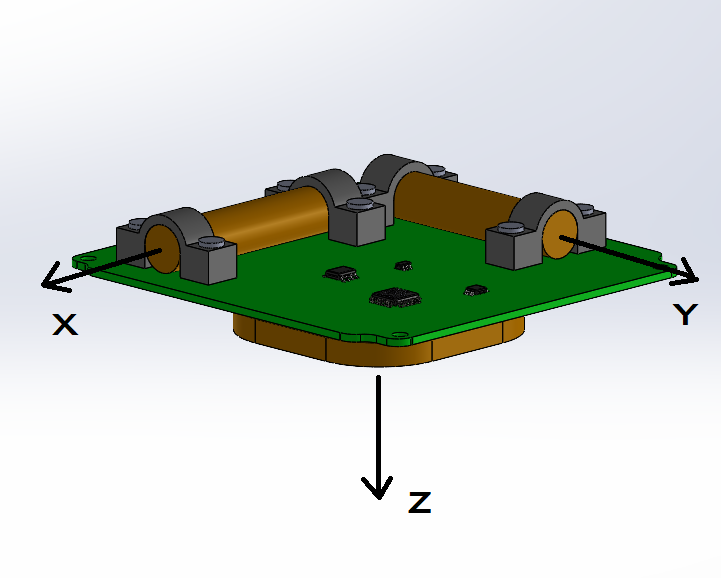
\includegraphics[width=5cm]{figures/Image axles.png}
                \end{center}
            \end{figure}
        \end{column}
    \end{columns}

\end{frame}

\begin{frame}{Dimensioning: Magnetic Core}
    
     \begin{columns}[t]
        \begin{column}[t]{0.5\textwidth}
            \begin{itemize}
                \item Only two coils with magnetic core
                \item Magnetic core with low coercive force and high relative permeability (>2000).
                \item Torque $=0.2 Am^2$ \textcolor{red}{TBC}.
            \end{itemize}
        \end{column}
        \begin{column}[t]{0.5\textwidth}
            \begin{figure}[!ht]
                \begin{center}
                    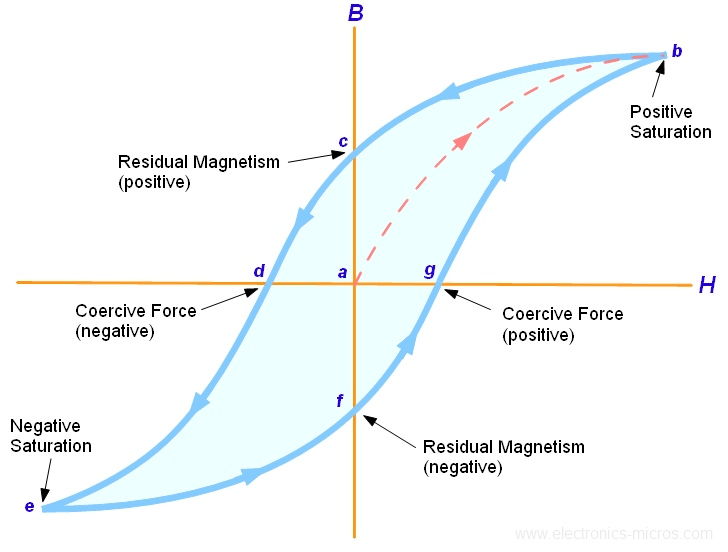
\includegraphics[width=5cm]{figures/hysteresis-loop.jpg}
                \end{center}
            \end{figure}
        \end{column}
    \end{columns}

\end{frame}

\begin{frame}{Dimensioning: Magnetorquer Material}
    
     \begin{columns}[t]
        \begin{column}[t]{0.5\textwidth}
            \begin{itemize}
                \item Magnetorquer core Material \textcolor{red}{TBD}

            \end{itemize}
        \end{column}
        \begin{column}[t]{0.5\textwidth}
            \begin{figure}[!ht]
                \begin{center}
                    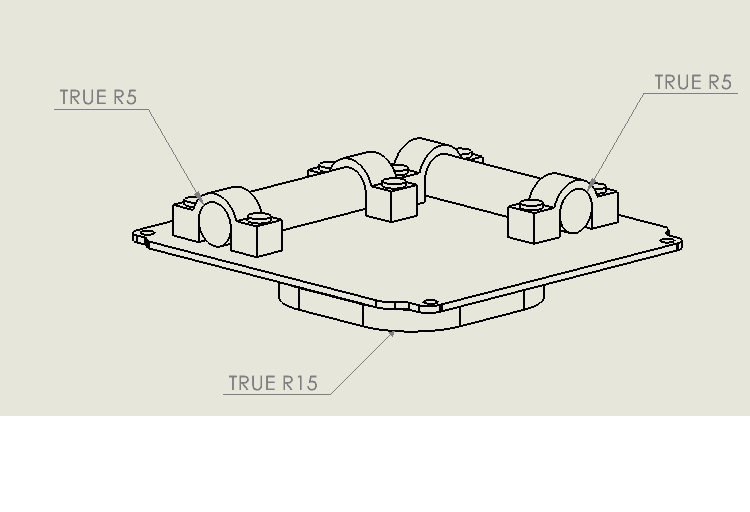
\includegraphics[width=5cm]{figures/desenho adcs.png}
                \end{center}
            \end{figure}
        \end{column}
    \end{columns}

\end{frame}

\begin{frame}{Dimensioning: Magnetorquer Sizing (X; Y; Z)}
    
     \begin{columns}[t]
        \begin{column}[t]{0.5\textwidth}
            \begin{itemize}
                \item Coil in axle X:
                D: \textcolor{red}{TBD}
                L: \textcolor{red}{TBD}
                \item Coil in axle Y:
                D: \textcolor{red}{TBD}
                L: \textcolor{red}{TBD}
                \item Coil in axle Z:
                D: \textcolor{red}{TBD}
                L: \textcolor{red}{TBD}

            \end{itemize}
        \end{column}
        \begin{column}[t]{0.5\textwidth}
            \begin{figure}[!ht]
                \begin{center}
                    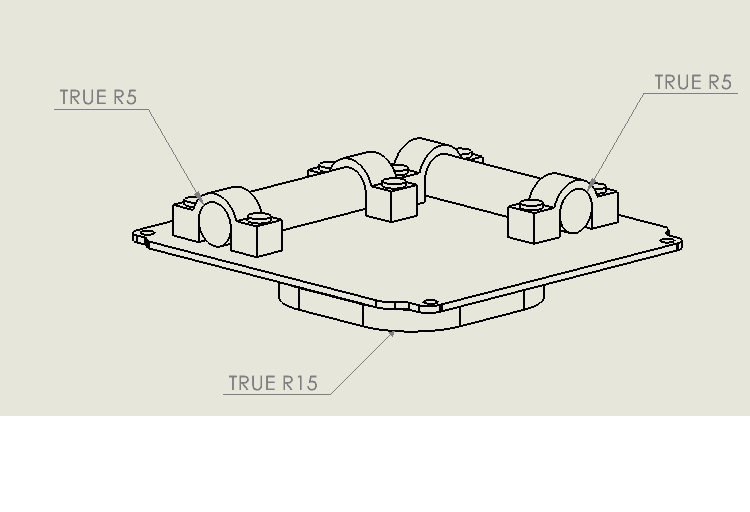
\includegraphics[width=5cm]{figures/desenho adcs.png}
                \end{center}
            \end{figure}
        \end{column}
    \end{columns}

\end{frame}

\begin{frame}{Final result}
\begin{figure}[!ht]
        \begin{center}
            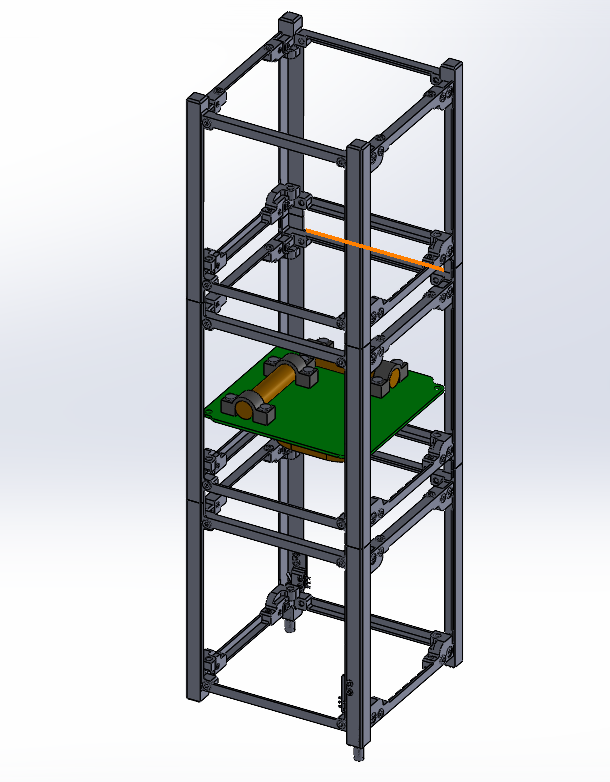
\includegraphics[width=5.6cm]{figures/Structure with ADCS.png}
        \end{center}
    \end{figure}

\end{frame}

    \section{Management}

        %
% management.tex
%
% Copyright (C) 2022 by SpaceLab.
%
% Camera Payload Preliminary Design Review
%
% This work is licensed under the Creative Commons Attribution-ShareAlike 4.0
% International License. To view a copy of this license,
% visit http://creativecommons.org/licenses/by-sa/4.0/.
%

%
% \brief Project management slides.
%
% \author Gabriel Mariano Marcelino <gabriel.mm8@gmail.com>
% \author Vitória Beatriz Bianchin <vitoriabbianchin@gmail.com>
% \author Caique Sales de Miranda Gomes <kiqsmg@gmail.com>
%
% \version 0.1.0
%
% \date 2022/06/24
%


\begin{frame}{Project Management}

    \begin{itemize}
        \item Activities and tasks: GitHub issues/project
        \vspace{0.25cm}
        \item Periodic meetings
        \vspace{0.25cm}
        \item Source files and versioning control: Git/GitHub repository (\href{https://github.com/spacelab-ufsc/adcs}{\textcolor{blue}{https://github.com/spacelab-ufsc/adcs}}) with five development branches:
            \begin{itemize}
                \item \textit{dev\_doc}: Documentation
                \item \textit{dev\_hardware}: Hardware project
                \item \textit{dev\_firmware}: Firmware project
                \item \textit{dev\_mechanical}: Mechanical project
%                \item \textit{dev\_validation}: Validation setup sources
            \end{itemize}
    \end{itemize}

\end{frame}

% #########################################################################
% #########################################################################

\begin{frame}{Product Tree}

    \begin{figure}[!ht]
        \begin{center}
            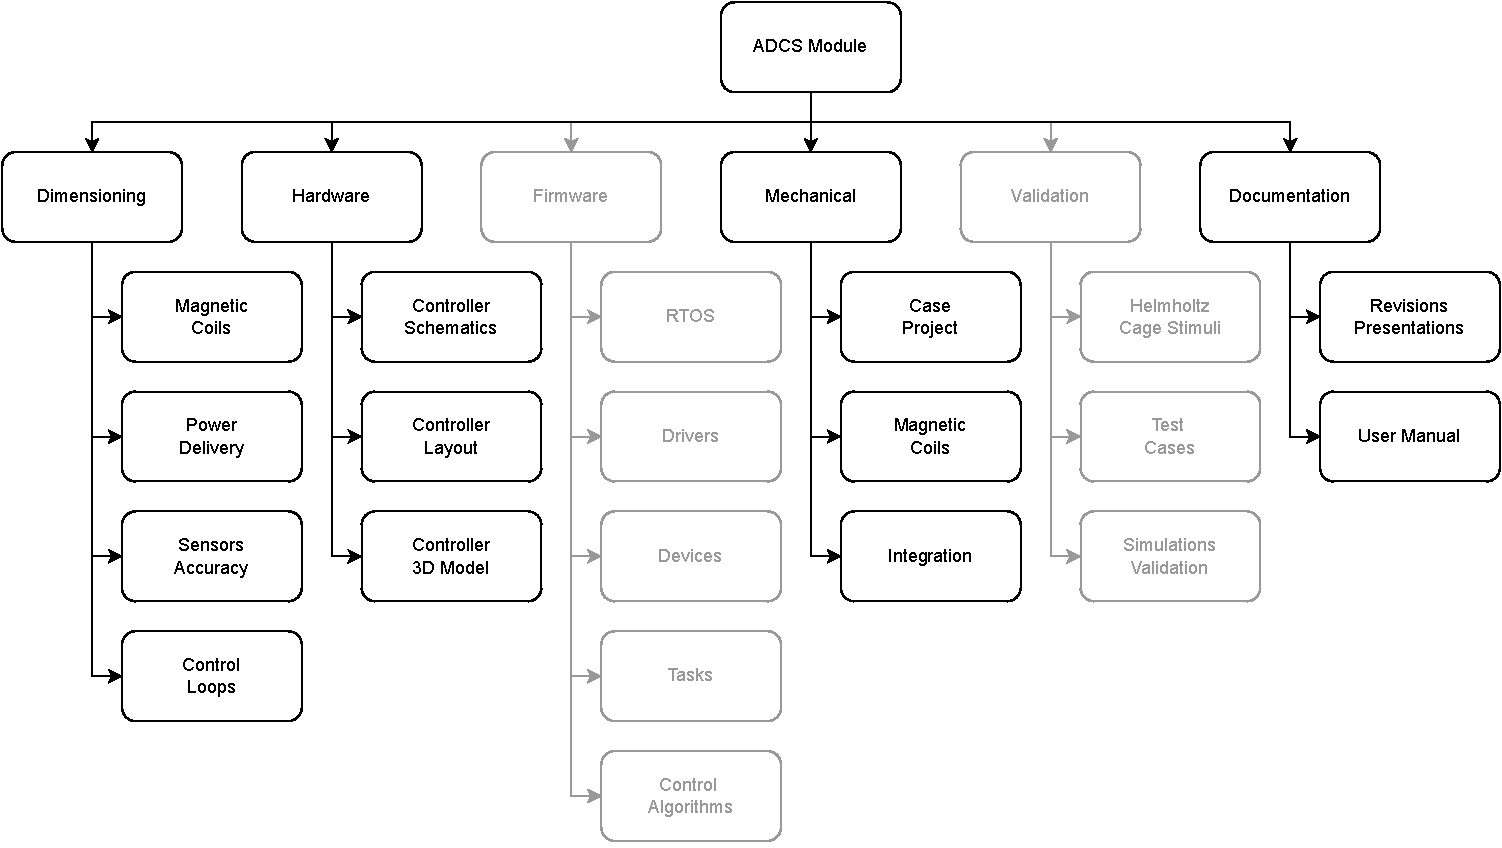
\includegraphics[width=11cm]{figures/product-tree-adcs.pdf}
        \end{center}
    \end{figure}

\end{frame}

% #########################################################################
% #########################################################################

\begin{frame}{Schedule}

\begin{table}[!htb]\tiny
    \centering
    \label{tab:schedule}
    \begin{tabular}{lC{0.15cm}C{0.15cm}C{0.15cm}C{0.15cm}C{0.15cm}C{0.15cm}C{0.15cm}C{0.15cm}C{0.15cm}C{0.15cm}C{0.15cm}C{0.15cm}}
        \toprule[1.5pt]
        \multirow{2}{*}{\textbf{Activity}} & \multicolumn{12}{c}{\textbf{Week}} \\
                          & W1 & W2 & W3 & W4 & W5 & W6 & W7 & W8 & W9 & W10 & W11 & W12 \\
        \midrule                      % 1   2   3   4   5   6   7   8   9   10  11  12
        Project definition            & X &   &   &   &   &   &   &   &   &   &   &     \\
        Bibliographical review        & X &   &   &   &   &   &   &   &   &   &   &     \\
        Project dimensioning          &   & X & X &   &   &   &   &   &   &   &   &     \\
        Component selection           &   & X & X &   &   &   &   &   &   &   &   &     \\
        \textbf{PDR}                  &   &   & \textbf{X} &   &   &   &   &   &   &   &   &     \\
        Mechanical design             &   &   & X & X &   &   &   &   &   &   &   &     \\
        Controller schematics         &   &   & X & X & X &   &   &   &   &   &   &     \\
        Components aquisiton          &   &   &   & X & X & X & X & X &   &   &   &     \\
        Controller PCB layout         &   &   &   & X & X & X & X &   &   &   &   &     \\
        Mockup fabrication            &   &   &   &   &   &   & X &   &   &   &   &     \\
        \textbf{CDR}                  &   &   &   &   &   &   & \textbf{X} &   &   &   &   &     \\
        Controller PCB fabrication    &   &   &   &   &   &   &   & X & X & X & X &     \\
        Case fabrication              &   &   &   &   &   &   &   & X & X &   &   &     \\
        User manual preparation       &   &   &   &   &   &   &   &   & X & X & X &     \\
        Preliminary Electrical tests  &   &   &   &   &   &   &   &   &   &   & X &     \\
        Mechanical integration        &   &   &   &   &   &   &   &   &   &   & X &     \\
        \textbf{AR}                   &   &   &   &   &   &   &   &   &   &   &   & \textbf{X}   \\
        \bottomrule[1.5pt]
    \end{tabular}
\end{table}

{\footnotesize Schedule changes from the original presentation (besides PDR, CDR, and AR):\\5.3:W2, 5.5:W5, 5.7:W9, 5.9:W13}

\end{frame}

% #########################################################################
% #########################################################################

\begin{frame}{Team}

    \begin{table}[!htb]
        \centering
        \label{tab:team}
        \begin{tabular}{ll}
            \toprule[1.5pt]
            \textbf{Role} & \textbf{Name} \\
            \midrule
            \multirow{2}{*}{Management/Support}   & André M. P. de Mattos \\
                                                  & Gabriel M. Marcelino \\
            \midrule
            Dimensioning                          & Matheus Wagner \\
            \midrule
            \multirow{4}{*}{Hardware design}      & Rebecca Q. Do Ó \\
                                                  & Bruno Benedetti \\
                                                  & Caique S. de M. Gomes \\
            \midrule
            Mechanical design                     & Caique S. de M. Gomes \\
            \bottomrule[1.5pt]
        \end{tabular}
    \end{table}

\end{frame}

% #########################################################################
% #########################################################################

\begin{frame}{Cost Estimation\footnote{2 units.}}

\begin{table}[!htb]\scriptsize
    \centering
    \label{tab:cost-estimation}
    \begin{tabular}{lccc}
        \toprule[1.5pt]
        \textbf{Item} & \textbf{Unit (US\$)} & \textbf{Quantity} & \textbf{Total (US\$)} \\
        \midrule
        STM32F103C8T6         & 7.31  & 2  & 14.62 \\
        TCAN330GD             & 3.89  & 2  & 7.78 \\
        Sensors               & 10.00 & 2  & 20.00 \\
        H-Bridge              & 2.00  & 2  & 4.00 \\
        Copper wire           & 10.00 & 1  & 10.00 \\
        Magnetic core         & 10.00 & 4  & 40.00 \\
        Passive components    & 5.00  & 1  & 5.00 \\
        PCB                   & 0.50  & 10 & 5.00 \\
        \midrule
        Total          & \multicolumn{3}{c}{106.40\footnote{Prices in August 2022, without delivery rates or taxes.}} \\
        \bottomrule[1.5pt]
    \end{tabular}
\end{table}

\end{frame}
        
\begin{frame}{Project Management}

    \begin{itemize}
        \item Activities and tasks: GitHub issues/project
        \vspace{0.25cm}
        \item Periodic meetings
        \vspace{0.25cm}
        \item Source files and versioning control: Git/GitHub repository (\href{https://github.com/spacelab-ufsc/adcs}{\textcolor{blue}{https://github.com/spacelab-ufsc/adcs}}) with five development branches:
            \begin{itemize}
                \item \textit{dev\_doc}: Documentation
                \item \textit{dev\_hardware}: Hardware project
                \item \textit{dev\_firmware}: Firmware project
                \item \textit{dev\_mechanical}: Mechanical project
%                \item \textit{dev\_validation}: Validation setup sources
            \end{itemize}
    \end{itemize}

\end{frame}
        
\begin{frame}{Documentation}

    \begin{itemize}
        \item User manual (PDF)
        \vspace{0.4cm}
        \item This presentation
        \vspace{0.4cm}
        \item Schematics
        \vspace{0.4cm}
    \end{itemize}

\end{frame}

\begin{frame}{Product Tree}

    \begin{figure}[!ht]
        \begin{center}
            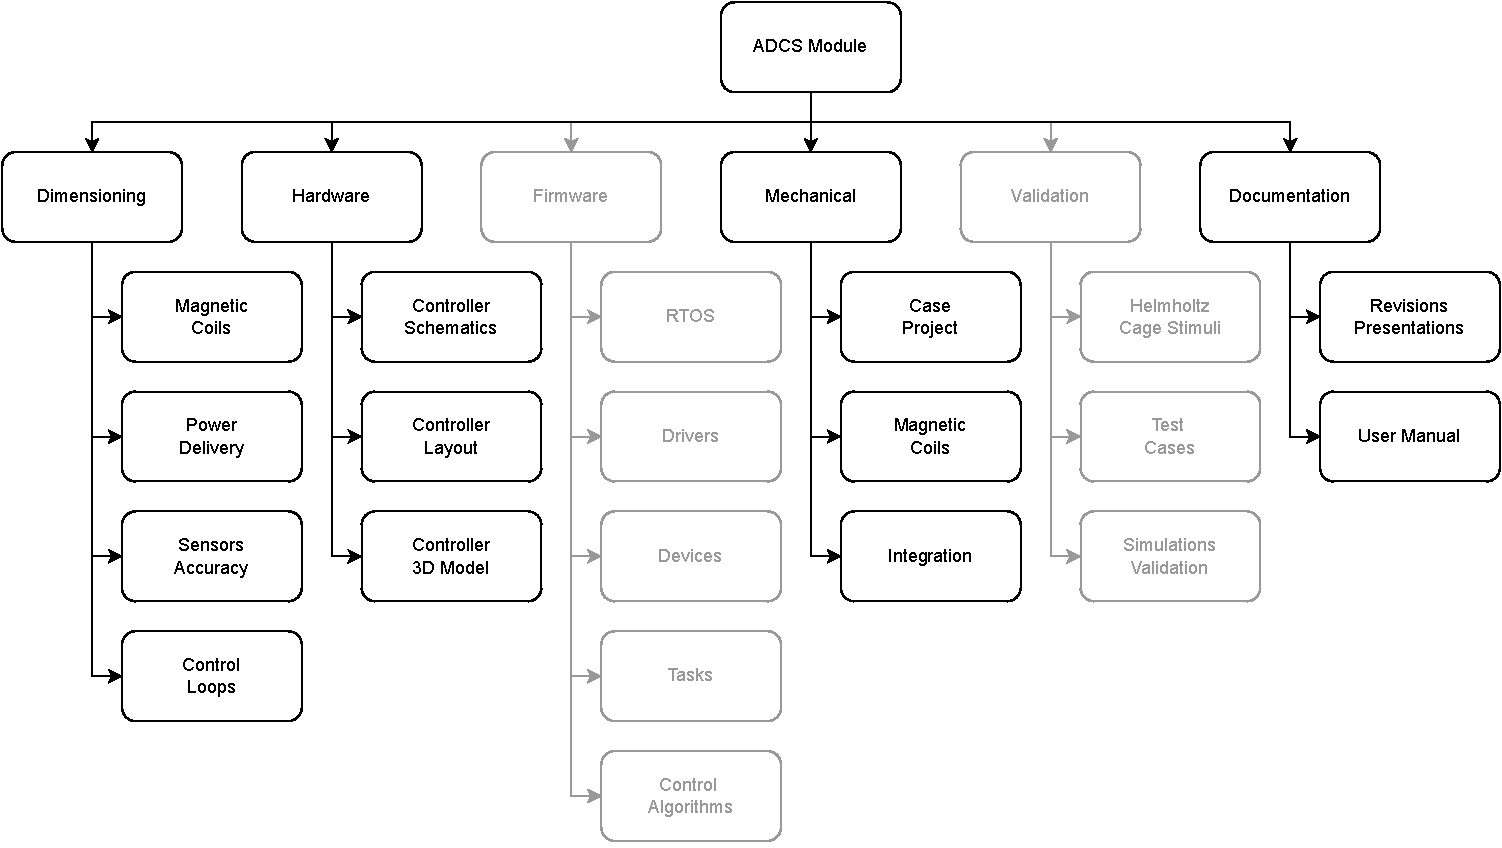
\includegraphics[width=11cm]{figures/product-tree-adcs.pdf}
        \end{center}
    \end{figure}

\end{frame}

\begin{frame}{Schedule}

\begin{table}[!htb]\tiny
    \centering
    \label{tab:schedule}
    \begin{tabular}{lC{0.15cm}C{0.15cm}C{0.15cm}C{0.15cm}C{0.15cm}C{0.15cm}C{0.15cm}C{0.15cm}C{0.15cm}C{0.15cm}C{0.15cm}C{0.15cm}}
        \toprule[1.5pt]
        \multirow{2}{*}{\textbf{Activity}} & \multicolumn{12}{c}{\textbf{Week}} \\
                          & W1 & W2 & W3 & W4 & W5 & W6 & W7 & W8 & W9 & W10 & W11 & W12 \\
        \midrule                      % 1   2   3   4   5   6   7   8   9   10  11  12
        Project definition            & X &   &   &   &   &   &   &   &   &   &   &     \\
        Bibliographical review        & X &   &   &   &   &   &   &   &   &   &   &     \\
        Project dimensioning          &   & X & X &   &   &   &   &   &   &   &   &     \\
        Component selection           &   & X & X &   &   &   &   &   &   &   &   &     \\
        \textbf{PDR}                  &   &   & \textbf{X} &   &   &   &   &   &   &   &   &     \\
        Mechanical design             &   &   & X & X &   &   &   &   &   &   &   &     \\
        Controller schematics         &   &   & X & X & X &   &   &   &   &   &   &     \\
        Components aquisiton          &   &   &   & X & X & X & X & X &   &   &   &     \\
        Controller PCB layout         &   &   &   & X & X & X & X &   &   &   &   &     \\
        Mockup fabrication            &   &   &   &   &   &   & X &   &   &   &   &     \\
        \textbf{CDR}                  &   &   &   &   &   &   & \textbf{X} &   &   &   &   &     \\
        Controller PCB fabrication    &   &   &   &   &   &   &   & X & X & X & X &     \\
        Case fabrication              &   &   &   &   &   &   &   & X & X &   &   &     \\
        User manual preparation       &   &   &   &   &   &   &   &   & X & X & X &     \\
        Preliminary Electrical tests  &   &   &   &   &   &   &   &   &   &   & X &     \\
        Mechanical integration        &   &   &   &   &   &   &   &   &   &   & X &     \\
        \textbf{AR}                   &   &   &   &   &   &   &   &   &   &   &   & \textbf{X}   \\
        \bottomrule[1.5pt]
    \end{tabular}
\end{table}

{\footnotesize Schedule changes from the original presentation (besides PDR, CDR, and AR):\\5.3:W2, 5.5:W5, 5.7:W9, 5.9:W13}

\end{frame}

\begin{frame}{Team}

    \begin{table}[!htb]
        \centering
        \label{tab:team}
        \begin{tabular}{ll}
            \toprule[1.5pt]
            \textbf{Role} & \textbf{Name} \\
            \midrule
            \multirow{2}{*}{Management/Support}   & André M. P. de Mattos \\
                                                  & Gabriel M. Marcelino \\
            \midrule
            Dimensioning                          & Matheus Wagner \\
            \midrule
            \multirow{4}{*}{Hardware design}      & Rebecca Q. Do Ó \\
                                                  & Bruno Benedetti \\
                                                  & Caique S. de M. Gomes \\
            \midrule
            Mechanical design                     & Caique S. de M. Gomes \\
            \bottomrule[1.5pt]
        \end{tabular}
    \end{table}

\end{frame}

\begin{frame}{Cost Estimation\footnote{2 units.}}

\begin{table}[!htb]\scriptsize
    \centering
    \label{tab:cost-estimation}
    \begin{tabular}{lccc}
        \toprule[1.5pt]
        \textbf{Item} & \textbf{Unit (US\$)} & \textbf{Quantity} & \textbf{Total (US\$)} \\
        \midrule
        STM32F303RCT6         & 8.86     & 2  & 17.72  \\
        TCAN330GD             & 3.89  & 2  & 7.78 \\
        ina226                & 9.24  & 8  & 73.92\\
        TMP100                & 2.68  & 8  & 21.44\\
        I3G4250DTR            & 10.98 & 2  & 10.98 \\
        MMC5983MA             & 4.44  & 2  & 8.88 \\
        DRV8834PWP            & 3.62  & 6  & 28.96 \\
        Copper wire           & -     & 1  & - \\
        Magnetic core         & -     & 4  & - \\
        Passive components    & 5.00  & 1  & 5.00 \\
        PCB                   & 0.50  & 10 & 5.00 \\
        TPS3823-50DBVR        & 1.59  & 2 & 3.18 \\
        \midrule
        Total          & \multicolumn{3}{c}{204.04\footnote{Prices in August 2022, without delivery rates or taxes.}} \\
        \bottomrule[1.5pt]
    \end{tabular}
\end{table}

\end{frame}

    \sectionpic{Thanks!}{figures/brazil-south.jpeg}

\end{document}
